\scanpage{45}
comme on voit ainsi. \deleted{On fixe $u_0\in Z'_s$,
et une origine $i_0\in I_s$, d'où $i_1\ldots i_{\nu_s-1}$ donnés
par}
\[\deleted{i_\nu=u_0^{\nu}i_0}\]
\deleted{Soit $\omega_\nu$ l'une des deux orientations de $D_{i_\nu}$ i.e. la
\deleted{\unsure{un de|l'un}} fibre de $i_\nu$ dans (26), alors $u$
est connue}

On fixe $u_0\in Z_s^{\unsure{\prime|1}}$, i.e. une
orientation du polygone d'ens de
sommets $I_s$, pour chaque
$i\in I_s$, on doit se donner une
bijection \inserted{$\alpha_i$} de $\unsure{\vec I_i|\vec I_{2i}}$ la fibre de
$\vec I_s$ en $i$, \{i.e. de l'ens \inserted{$\omega_i$} des
deux orientations de $D_i$\}
\figure{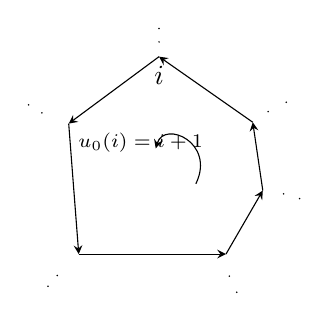
\begin{tikzpicture}[scale=.85,>=stealth]
\coordinate (t) at (0,2.0); \coordinate (l) at (-1.35,1.0);
\coordinate (bl) at (-1.2,-.95); \coordinate (br) at (1.0,-.95);
\coordinate (r) at (1.55,0); \coordinate (tr) at (1.4,1.02);
\draw[->] (t)--(l); \draw[->] (l)--(bl); \draw[->] (bl)--(br);
\draw[->] (br)--(r); \draw[->] (r)--(tr); \draw[->] (tr)--(t);
\draw[->] (.55,.1) .. controls (.85,.72) and (.08,1.05) .. (-.05,.63);
\node[below] at (t) {$i$}; \node[below right,font=\scriptsize] at (l) {$u_0(i)=i+1$};
\foreach \x/\y in {0/2.22,0/2.42,-1.75/1.16,-1.95/1.28,-1.52/-1.27,-1.66/-1.43,1.05/-1.28,1.16/-1.52,1.86/-.05,2.1/-.12,1.63/1.18,1.9/1.32}{\fill (\x,\y) circle (.013);}
\end{tikzpicture}}
avec $\omega_j$ où $j=u_0(i)$ est le sommet suivant $i$
— ce qui, pour $i$ fixé, fait 2 choix, donc
en tout, en apparence, $2^{\nu_s}$ choix. Mais on
veut que la permutation $u$ de $\vec I_s$ obtenue
soit une permutation circulaire, i.e. \deleted{soit}
transitive ; si on fixe $i_0\in I$ \inserted{et on pose $i_{\unsure{\alpha|\nu}}=u_0^{\unsure{\nu|\alpha}}(i_0)$}
cela signifie que
les choix de $\alpha_{i_0},\alpha_{i_1},\ldots,\alpha_{i_{\nu_s-2}}$
\margin{$\nu=\nu_s$}
\[\omega_{i_0}\mathrel{\mathop{\rule{1.8em}{.4pt}}\limits^{\substack{\alpha_{i_0}\\\sim}}}\omega_{i_1}
\mathrel{\mathop{\longrightarrow}\limits^{\substack{\alpha_{i_1}\\\sim}}}\omega_{i_2}\quad\ldots\quad
\omega_{i_{\nu_s-2}}\mathrel{\mathop{\longrightarrow}\limits^{\substack{\alpha_{i_{\nu_s-2}}\\\sim}}}\omega_{i_{\nu_s-1}}\tag*{(28)}\]
déterminent le choix du dernier $\alpha_{i_{\nu-1}}:\omega_{i_{\nu-1}}\mathrel{\mathop{\rule{1.6em}{.4pt}}\limits^{\sim}}\omega_{i_\nu}=\omega_{i_0}$
par la condition qu'il soit \uline{distinct} \inserted{(i.e. que ce soit l'\uline{opposé})} \deleted{du composé}
l'inverse du composé des bij. précédentes.
\deleted{Dans le cas où}
% archive sheet number: 44
